\documentclass{standalone}
\usepackage{tikz}
\usepackage{ctex,siunitx}
\usepackage{tkz-euclide}
\usepackage{amsmath}
\usetikzlibrary{patterns, calc}
\usetikzlibrary {decorations.pathmorphing, decorations.pathreplacing, decorations.shapes,}
\begin{document}
\small
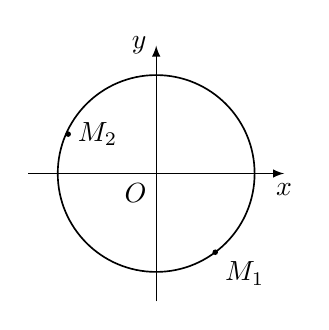
\begin{tikzpicture}[>=latex,scale=0.25]
  % \useasboundingbox(0,-0.2)rectangle(3,0.5);
  \draw[thin,->](-6.5,0)--(6.5,0)node[below]{$x$};
  \draw[thin,->](0,-6.5)--(0,6.5)node[left]{$y$};
  \node at (0,0)[below left]{$O$};
  \draw[semithick](0,0)circle(5);
  \fill(3,-4)circle(4pt)node[below right]{$M_1$};
  \fill(-4.47,2)circle(4pt)node[right]{$M_2$};
\end{tikzpicture}
\end{document}